\documentclass[11pt]{jarticle}
\usepackage[a4paper, margin=20mm]{geometry}
\usepackage{wrapfig}
\usepackage{jtygm}
\usepackage{listings}
\usepackage[usenames, dvipsnames]{color}
\usepackage[dvipdfmx]{graphicx}
\usepackage{keystroke}
\usepackage{menukeys}
\usepackage{siunitx}

\newcommand\secref[1]{\mbox{\ref{#1}節}}
\newcommand\gamename{サムライジョッキー}

\title{{\gamename}ゲームルール}
\author{情報処理学会プログラミングコンテスト委員会}
\date{2017/12/26}

\begin{document}
\maketitle

\begin{abstract}
  SamurAI Coding 2017--18 に用いるゲームのルールを述べる.
  % このルール案は暫定版であり, 詳細については今後の改訂の可能性がある.
\end{abstract}

\section{ゲームの概要}
AIの制御するふたりのプレイヤがスタート位置から開始し,障害物が設置され
たレースコース上でステップごとに位置を変えながら,ゴールに早く到達する
ことを競うゲームである.

1ゲームは,同じレースコースを用い両プレイヤのスタート位置を交換した2レー
スからなる. 両レースのゴールタイムの合計が短い方がゲームの勝者である.
合計タイムが同一である場合は,そのゲームは引き分けである.

\begin{wrapfigure}{r}{0.38\columnwidth}
  \vspace{-2cm}
  \centering
  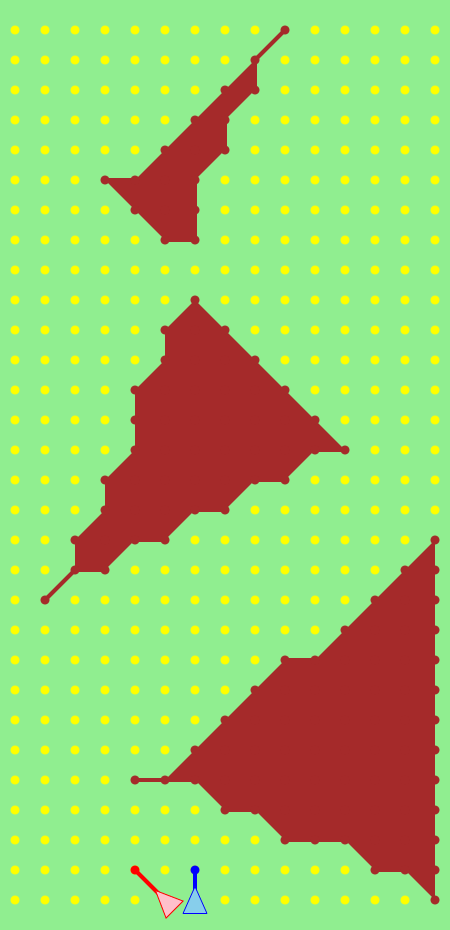
\includegraphics[width=0.35\columnwidth, natwidth=450, natheight=930]{racecourse.png}
  \caption{レースコースの例}
  \label{fig:course}
\end{wrapfigure}

\section{レースコース}
レースコースは2次元格子状であり,ゲーム毎に大きさや障害物の位置が異なる.
以下ではレースコースの幅を$w$,コース長を$l$とし,
各格子点の位置の座標を $(x,y)$ ($0\le x < w, 0\le y$) とする.

コース上の格子点の一部は{\bf 障害点}である.  障害点あるいは縦横斜めに
隣接するふたつの障害点を結んだ線分を{\bf 障害物}と呼ぶ. 障害物は固定さ
れており,レース中に動くことはない.  障害物を飛び越すことはできないの
で,障害物に囲まれた領域に入ることはできない.

プレイヤを制御するAIプログラム (以下単に{\bf AI}と呼ぶ) に与えられる障
害物の情報は,プレイヤの視界の範囲内のもの,すなわちプレイヤの位置の前
後一定範囲の$y$座標にあるものについてのみである. 加減速は限定された範
囲でしかできないので,速度を上げ過ぎると障害物を避けられなくなる可能性
がある.

図\ref{fig:course}にレースコースの例を示す. 茶色の小円は障害点,線分や
塗りつぶした領域は障害物およびそれらに囲まれた領域である.

レース中,両プレイヤはいずれかの相異なる格子点にある.  レース開始時の
両プレイヤの位置の$x$座標は異なり,$y$座標は$0$である.  両プレイヤはス
テップごとに位置を変えて行き,コース長$l$以上の$y$座標の地点に達したら
ゴールしたことになる.

コースには行き止まりがないものとする. レース開始時の両プレイヤの位置か
ら到達可能なコース内のどの格子点からも,十分小さい速度で移動すれば,一
度も$y$座標を減らすことなく障害物やコース端にぶつからずに$y$座標がより
大きい点に移動できる.

\section{レースの進行}\label{sec:race_process}
各レースでは,ステップごとにAIにレースの状況についての情報を与え,それ
に対するAIからの応答である加減速指示に従ってレースの状況を更新すること
を繰り返す.  レース中に両プレイヤが同時に同じ位置を占めることはない.

ステップは0から1ずつ進み,両プレイヤ共にゴールまたは失格
(\secref{sec:disqualification})すればレースは終了である. ただし,制限
ステップ数に達してもゴールしないプレイヤがある場合,その時点でレースは
終了し,ゴールに達していないプレイヤは失格となる.

\subsection{考慮時間}\label{sec:consideration_time}
AIが1レースで使える{\bf 考慮時間}の合計には,制限を設ける. 考慮時間は
ゲーム管理プログラムがプレイヤに情報を送信し終わってから,プレイヤから
の応答を受信し終わるまでの実時間である.  考慮時間の合計が制限値を超え
たプレイヤは失格となる.
%\footnote{考慮時間の制限値は未定だが,数十秒程度となるだろう.}

\subsection{プレイヤの状態と加減速指示}
プレイヤは各ステップの開始時において{\bf 位置} $(x, y)$ と{\bf 速度}
$(v_\mathrm{x}, v_\mathrm{y})$ を持つ.

AIはステップごとに速度を変更する{\bf 加速度} $(a_\mathrm{x}, a_\mathrm{y})$を指定する.
$a_\mathrm{x}, a_\mathrm{y}$は各々$-1, 0, 1$のいずれかである.

後述するコースアウトや衝突によって動けない場合を除き,次ステップのプレ
イヤの位置の座標は $(x+v_\mathrm{x}+a_\mathrm{x}, y+v_\mathrm{y}+a_\mathrm{y})$ となる. この位置を以下では
次ステップにおける{\bf 予定位置}と呼ぶ. また,次ステップにおけるプレイ
ヤの速度はコースアウトや衝突の有無に関わらず $(v_\mathrm{x}+a_\mathrm{x}, v_\mathrm{y}+a_\mathrm{y})$ とな
る.

\begin{wrapfigure}{R}{0.28\columnwidth}
  \vspace{-1cm}
  \centering
  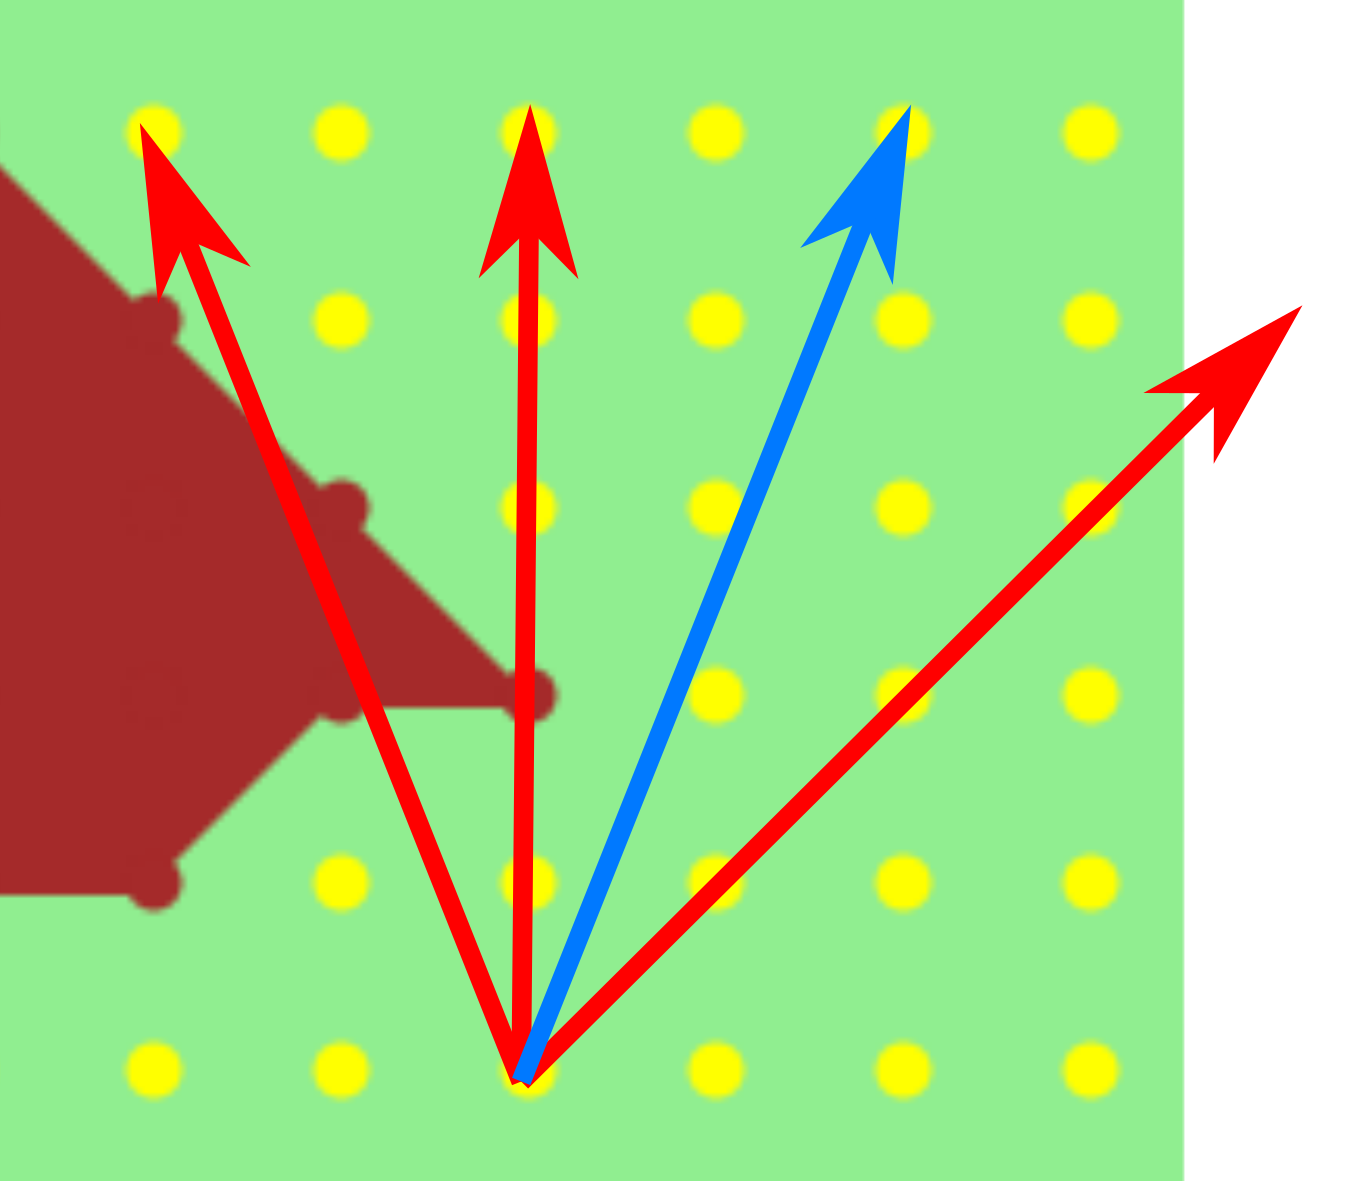
\includegraphics[width=0.26\columnwidth, natwidth=1358, natheight=1181]{courseout.png}
  \caption{コースアウト}
  \label{fig:courseout}
  赤い動線はコースアウト
  \vspace{-1cm}
\end{wrapfigure}

\subsection{動線とコースアウト}

プレイヤの位置と次ステップにおける予定位置を両端とする線分を,このプレ
イヤの当該ステップでの{\bf 動線}と呼ぶ.

以下の場合,当該プレイヤは{\bf コースアウト}を生じているという.
\begin{itemize}
\item
  予定位置がコース外に出る,すなわち予定位置の座標$(x,y)$が$0 \le x <
  w$ かつ $0 \le y$ を満たさない場合
\item
  動線が障害物と交差あるいは接触する場合
\end{itemize}
コースアウトしたプレイヤの次ステップでの位置は元のままになる.  速度に
ついてはコースアウトしなかった場合と同じ加速度が適用される.

\begin{wrapfigure}{R}{0.32\columnwidth}
  \centering
  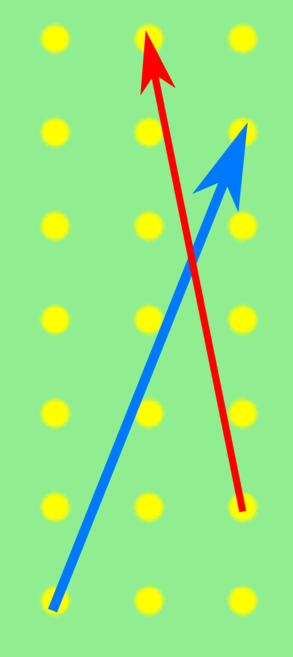
\includegraphics[scale=0.2, natwidth=293, natheight=657]{collision.png}
  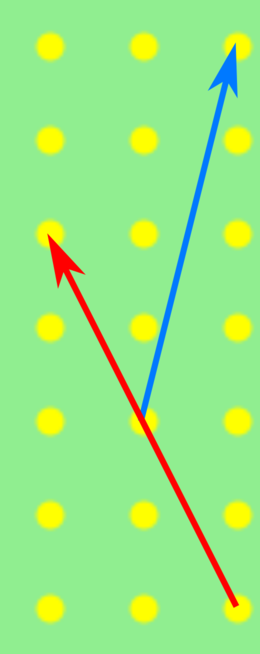
\includegraphics[scale=0.183, natwidth=288, natheight=657]{cropped.png}
  \caption{衝突}
  \label{fig:collision}
  いずれも青い動線のプレイヤが優先権を持つ
  \vspace{-1.5cm}
\end{wrapfigure}

\subsection{衝突と優先権}
コースアウトがない場合に,両プレイヤの動線が交差あるいは接触する場合,
{\bf 衝突}が生じたという.

衝突が生じた場合は,{\bf 優先権}を持つプレイヤの次ステップの位置は予定
位置に,優先権のないプレイヤの位置は元のままになる.  いずれのプレイヤ
についても,次ステップの速度は衝突しなかった場合と同じ$(v_\mathrm{x}+a_\mathrm{x},
v_\mathrm{y}+a_\mathrm{y})$となる.

優先権を持つのは,位置の$y$座標がより小さいプレイヤである.  $y$座標が
同一である場合,位置の$x$座標がより小さいプレイヤが優先権を持つ. ただ
し,動線が相手プレイヤの動作前の位置に達するか通過する場合は,優先権
が相手プレイヤに移る.

両プレイヤとも互いに相手の位置に達するか通過するような動線を持つ場合は,
両者とも優先権を失い,次のステップでの位置は元のままとなる.

\subsection{ゴールタイム}
プレイヤがステップ$s$で座標$(x, y)$の位置にあり,次ステップで位置$(x',
y')$に達し,$y'\ge l$ ($l$ はコース長) であるとき,そのプレイヤはゴー
ルしたものとされる.  このときゴールタイムは$s + (l-y)/(y'-y)$で与えられる.

コースアウトしたプレイヤ,あるいは衝突を起こし優先権を持たないプレイヤ
は,たとえ予定位置の$y$座標がコース長以上であっても,次ステップの位置
は元の位置のままとなるので,そのステップではゴールしない.
\footnote{ゴール上やゴールより先に障害物が存在することもあるので注意されたい.}

ゴール時,相手プレイヤがゴールも失格もしていなければ,ゴールしたプレイ
ヤをコースから取り除いた状態でレースを継続する.

\subsection{失格}\label{sec:disqualification}
プレイヤは以下のいずれかを行った場合,失格となる.
\begin{itemize}
\item 制限ステップ数に達してもゴールできなかった(\secref{sec:race_process}冒頭).
\item 考慮時間の合計が制限値を超えた(\secref{sec:consideration_time}).
\item \secref{sec:output_init}や\secref{sec:output_step}の規定に反する出力を行った.
\end{itemize}

失格時,相手プレイヤがゴールも失格もしていなければ,失格したプレイヤを
コースから取り除いた状態でレースを継続する.失格したプレイヤのゴールタ
イムは制限ステップ数の2倍とする.

なお,失格の範囲は当該レース内に限られ,次以降のレースには通常通り参加
できる.

\section{AIの動作}
AIは初期化時にレース全体に関する情報を入力し,初期化終了を示す応答を出
力する. ステップごとにはレース状況の情報を入力し,応答として加速度指示
を出力する.

入力はただひとつの空白あるいは改行で区切った10進整数の並びである.
負の数にはマイナス符号を前置する.
初期化時の入力およびステップごとの入力の最後は必ず改行を置く.

AIの応答出力も空白あるいは改行で区切った10進整数の並びで,負の数にはマ
イナス符号を前置する.  {\bf 出力の最後には必ず改行を置く.}

\subsection{初期化時の入力}
初期化時のAIの入力は以下の項目がこの順に並ぶものである.
各項目の直後には改行が置かれ,1つの項目(1行)に含まれる複数の整数は{\bf ひとつの空白文字}で区切られる.
\begin{description}
\item[考慮時間$t_\mathrm{given}$] このレースで使える考慮時間をマイクロ秒単位の整数値として.
\item[制限ステップ数$s_\mathrm{max}$] ゴールまでのステップ数の上限を整数値として.
\item[コースサイズ] コースの幅$w$および長さ$l$を,ふたつの整数値として.
\item[視界$d$] 視界に入る$y$座標の範囲を整数値$d$として.
  位置$(x,y)$にあるプレイヤを制御するAIをに与えられる相手プレイヤや障害点の情報は,
  $y$座標が$y-d$から$y+d$の範囲 (両端を含む) にあるもののみが与えられる.
\end{description}

\makeatletter
\def\lst@visiblespace{$\color{Gray}{}_{
  \mbox{\kern.06em\vrule \@height.3ex}%
  \vbox{\hrule \@width.3em}%
  \hbox{\vrule \@height.3ex}}$}
\makeatother

\lstset{
  basicstyle=\ttfamily,
  frame = single,
  showspaces = true,
  escapeinside={<@}{@>},
  mathescape
}

初期化時の入力の形式を以下に示す.
\begin{lstlisting}
$t_\mathrm{given}$<@\tiny{\keys{\return}}@>
$s_\mathrm{max}$<@\tiny{\keys{\return}}@>
$w$ $l$<@\tiny{\keys{\return}}@>
$d$<@\tiny{\keys{\return}}@>
\end{lstlisting}

\subsection{初期化時の出力}\label{sec:output_init}
AIは初期化が終了したことを整数$0$ひとつ及び改行で伝える.

\begin{lstlisting}
0<@\tiny{\keys{\return}}@>
\end{lstlisting}

\subsection{ステップごとの入力情報}
ステップごとのAIの入力は以下の項目がこの順に並ぶものである.
各項目の直後には改行が置かれ,1つの項目に含まれる複数の整数は{\bf ひとつの空白文字}で区切られる.

\begin{description}
\item[ステップ$s$] 当該のステップの値を整数ひとつで与える.
\item[残り考慮時間$t_\mathrm{left}$] このレースで使える考慮時間の残りをマイクロ秒単位の整数値として.
\item[自プレイヤの状態] 当該のAIが制御するプレイヤの位置の$x$座標と$y$座標,速度の$x$成分$v_\mathrm{x}$と$y$成分$v_\mathrm{y}$の4整数.
\item[相手プレイヤの状態] 相手プレイヤの位置の$x$座標$x_\mathrm{e}$と$y$座標$y_\mathrm{e}$,速度の$x$成分$v_{\mathrm{x}_\mathrm{e}}$と$y$成分$v_{\mathrm{y}_\mathrm{e}}$の4整数.
  ただし,相手プレイヤの位置が視界の外であれば,$y$座標は$-1$,他は$0$になる.
\item[障害点] 視界内の各格子点が障害点であるか否かの情報で,
  $(2\times d+1)\times w$個の整数からなる. 視界内の$y-d$から$y+d$までの各$y$
  座標に対して$w$個の整数$o_{0,y}, o_{1,y}, \ldots, o_{w-1,y}$が,$y$
  座標の順に与えられる.  $o_{x,y}$が$1$ならば格子点$(x,y)$は障害点であ
  り,$0$ならばそうではない.  ただし,$y<0$であるコース外の格子点につ
  いては$1$が与えられる.なお障害点にのみ,$o_{w-1,y}$ と $o_{0,y+1}$ の間には
  空白文字でなく改行が区切りとして用いられる.すなわち $2\times d+1$ 行 $w$ 列が入力として与えられる.
\end{description}

ステップごとのAIの入力の形式を以下に示す.
\begin{lstlisting}
$s$<@\tiny{\keys{\return}}@>
$t_\mathrm{left}$<@\tiny{\keys{\return}}@>
$x$ $y$ $v_\mathrm{x}$ $v_\mathrm{y}$<@\tiny{\keys{\return}}@>
$x_\mathrm{e}$ $y_\mathrm{e}$ $v_{\mathrm{x}_\mathrm{e}}$ $v_{\mathrm{y}_\mathrm{e}}$<@\tiny{\keys{\return}}@>
$o_{0,y-d}$ $o_{1,y-d}$ $\ldots$ $o_{w-1,y-d}$<@\tiny{\keys{\return}}@>
$o_{0,y-d+1}$ $o_{1,y-d+1}$ $\ldots$ $o_{w-1,y-d+1}$<@\tiny{\keys{\return}}@>
$\ldots$
$o_{0,y+d}$ $o_{1,y+d}$ $\ldots$ $o_{w-1,y+d}$<@\tiny{\keys{\return}}@>
\end{lstlisting}

\subsection{ステップごとの出力}\label{sec:output_step}
AIは当該ステップの加速度$(a_\mathrm{x},a_\mathrm{y})$をふたつの整数で指定する.
$a_\mathrm{x}$および$a_\mathrm{y}$は$-1$, $0$, $1$のいずれかでなければならない.
各整数はひとつ以上の空白で区切り,最後に改行を置く.以下にステップごとの出力の形式を示す.ただし空白は2つ以上あってもよい.

\begin{lstlisting}
$a_\mathrm{x}$ $a_\mathrm{y}$<@\tiny{\keys{\return}}@>
\end{lstlisting}

\subsection{入出力例}

\begin{minipage}[t]{.6\textwidth}

\parindent=1zw

右に実際のAIへの入力例(黒字)およびAIからの出力例(赤字)を示す.これは,初期化から最初の2ステップまでの入出力である.

最初の4行は初期化時の入力であり,考慮時間,制限ステップ数,コースの幅,
長さおよび視界がそれぞれ$20,000\,\si{\micro\second}$,100,15,100,8
であることを示している.

この入力を受け取ったらAIは0と改行をを出力しなければならない.

以降はステップごとの入出力である.まず最初のステップについて,
現在のステップ数と残り考慮時間に対応する入力値がそれぞれ0,19981
となっていることから,このAIは初期化に$19\,\si{\micro\second}$かかり,
$19,981\,\si{\micro\second}$の考慮時間が残されていることがわかる.

次の2行には自プレイヤと相手プレイヤの状態が示されている.この例では,
自プレイヤの現在の位置$(x,y)$が$(5,0)$で
速度$(v_\mathrm{x},v_\mathrm{y})$は$(0,0)$であること,
および相手プレイヤの現在位置$(x_\mathrm{e},y_\mathrm{e})$が$(9,0)$で
速度$(v_{\mathrm{x}_\mathrm{e}},v_{\mathrm{y}_\mathrm{e}})$は$(0,0)$であることが確認できる.

次の17行(視界が$8$なので$(8 \times 2 + 1)$行)は視界内の各格子点が障害点か否かを示している.
この例では$y < 0$におけるすべての格子点が障害点であること,
および前方正面に大きな障害物があることがわかる.

AIはこの入力を受け取ったら,加速度$(a_\mathrm{x}, a_\mathrm{y})$を出力する必要がある.
この例では$(-1, 1)$を出力している.
すると,また次のステップの入力が第1ステップと同じ形式で与えられるので,
AIはまた加速度を出力する.これがレース終了まで繰り返される.

\end{minipage}
\hfill
\begin{minipage}[t]{.3\textwidth}
\begin{lstlisting}[aboveskip = -1.4\medskipamount, showspaces = false, basicstyle = \tiny, literate = {-}{-}1]
20000
100
15 100
8
<@\textcolor{red}{0}@>
0
19981
5 0 0 0
9 0 0 0
1 1 1 1 1 1 1 1 1 1 1 1 1 1 1
1 1 1 1 1 1 1 1 1 1 1 1 1 1 1
1 1 1 1 1 1 1 1 1 1 1 1 1 1 1
1 1 1 1 1 1 1 1 1 1 1 1 1 1 1
1 1 1 1 1 1 1 1 1 1 1 1 1 1 1
1 1 1 1 1 1 1 1 1 1 1 1 1 1 1
1 1 1 1 1 1 1 1 1 1 1 1 1 1 1
1 1 1 1 1 1 1 1 1 1 1 1 1 1 1
0 0 0 0 0 0 0 0 0 0 0 0 0 0 0
0 0 0 0 0 0 0 0 0 0 0 0 0 0 0
0 0 0 0 0 0 0 1 0 0 0 0 0 0 0
0 0 0 0 0 0 0 1 0 0 0 0 0 0 0
0 0 0 0 0 0 1 1 0 0 0 0 0 0 0
0 0 0 0 0 0 1 1 1 0 0 0 0 0 0
0 0 0 0 0 1 1 1 1 0 0 0 0 0 0
0 0 0 0 0 1 1 1 1 0 0 0 0 0 0
0 0 0 0 1 1 1 1 1 1 0 0 0 0 0
<@\textcolor{red}{-1 1}@>
1
19955
4 1 -1 1
8 1 -1 1
1 1 1 1 1 1 1 1 1 1 1 1 1 1 1
1 1 1 1 1 1 1 1 1 1 1 1 1 1 1
1 1 1 1 1 1 1 1 1 1 1 1 1 1 1
1 1 1 1 1 1 1 1 1 1 1 1 1 1 1
1 1 1 1 1 1 1 1 1 1 1 1 1 1 1
1 1 1 1 1 1 1 1 1 1 1 1 1 1 1
1 1 1 1 1 1 1 1 1 1 1 1 1 1 1
0 0 0 0 0 0 0 0 0 0 0 0 0 0 0
0 0 0 0 0 0 0 0 0 0 0 0 0 0 0
0 0 0 0 0 0 0 1 0 0 0 0 0 0 0
0 0 0 0 0 0 0 1 0 0 0 0 0 0 0
0 0 0 0 0 0 1 1 0 0 0 0 0 0 0
0 0 0 0 0 0 1 1 1 0 0 0 0 0 0
0 0 0 0 0 1 1 1 1 0 0 0 0 0 0
0 0 0 0 0 1 1 1 1 0 0 0 0 0 0
0 0 0 0 1 1 1 1 1 1 0 0 0 0 0
0 0 0 1 1 1 1 1 1 1 0 0 0 0 0
<@\textcolor{red}{0 1}@>
\end{lstlisting}
\end{minipage}

\subsection{情報の記憶}
ゲーム管理システムは,各ステップについて出力を終了したAIの動作を一時停
止し,次ステップの情報を与える際に動作を再開させる.  このため,ステッ
プの間に計算を進めることはできないが,変数値などの実行コンテキストは1
レースの間保持し続けることができる.

AIはファイル出力やネットワークアクセスができない環境で動作し,ゲーム管
理システムはレース毎にAIを初期状態から立ち上げ直す. このため,AIは複数
のレース間で情報を受け渡すことができない.

\begin{flushright}
以上
\end{flushright}

\end{document}
